\clearpage
\section*{5. Result and Analysis}
\label{sec:results}
\subsection*{5.1 Experimental parameters}

The campaign ran on 10 November 2026, on Ubuntu 26.04 LTS with kernel \texttt{7.0.0-42-generic}. GCC 15.2.0 and CMake 4.2.3 built both revisions \cite{ref13}.
Each access link has 1000 Mbit/s bandwidth and 5 ms delay in each direction.
The core link has 20 Mbit/s bandwidth and 25 ms delay in each direction.
Each shaped interface has a 1000-packet queue limit.
The nominal base RTT is 70 ms; the corresponding bandwidth-delay product is about 171 KiB.
Ping and qdisc checks verified both endpoint pairs.

Single-flow throughput uses the server's application bytes and connection duration.
Window and flight-size samples come from sender qlogs; final RTT comes from the server performance CSV.
Detailed graphs show repetition one. Tables use all three repetitions per mode.
The previous campaign is retained in a local backup, separate from these measurements.
\begin{center}
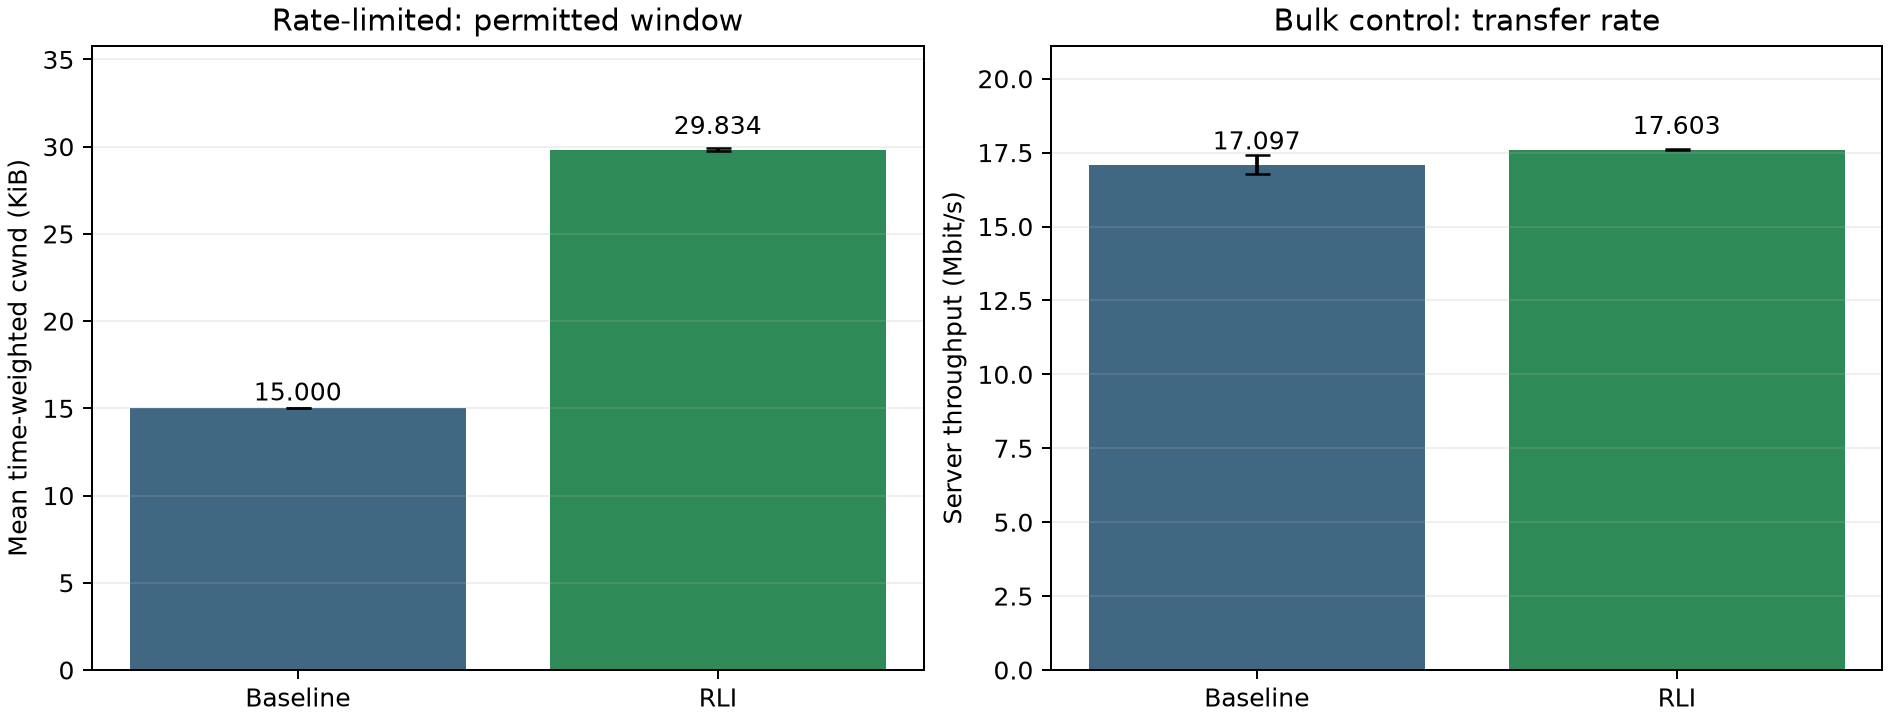
\includegraphics[width=\linewidth,height=.32\textheight,keepaspectratio]{images/native-overview.png}
\captionof{figure}{Fresh three-run means with sample standard-deviation bars for fixed-rate cwnd and bulk throughput.}
\end{center}

\subsection*{5.2 Fixed-rate workload}
\begin{center}\small\begin{tabular}{lrrrr}
Mode & Rate (Mbit/s) & Final cwnd (KiB) & Mean cwnd (KiB) & Final RTT (ms) \\ \hline
Original & 0.189391 & 15.00 & 15.00 & 71.794 \\
RLI & 0.189369 & 30.00 & 29.83 & 71.817 \\
\end{tabular}\end{center}

Each transfer delivers 480,000 bytes at an offered rate of approximately 192 kbit/s.
The largest observed RLI flight is 3426 bytes. The initialized 15 KiB maxFS sets the 30 KiB slow-start ceiling.
A larger permitted window does not increase the application's supply of data.
The experiment does not measure the completion time of a later burst.
\begin{center}
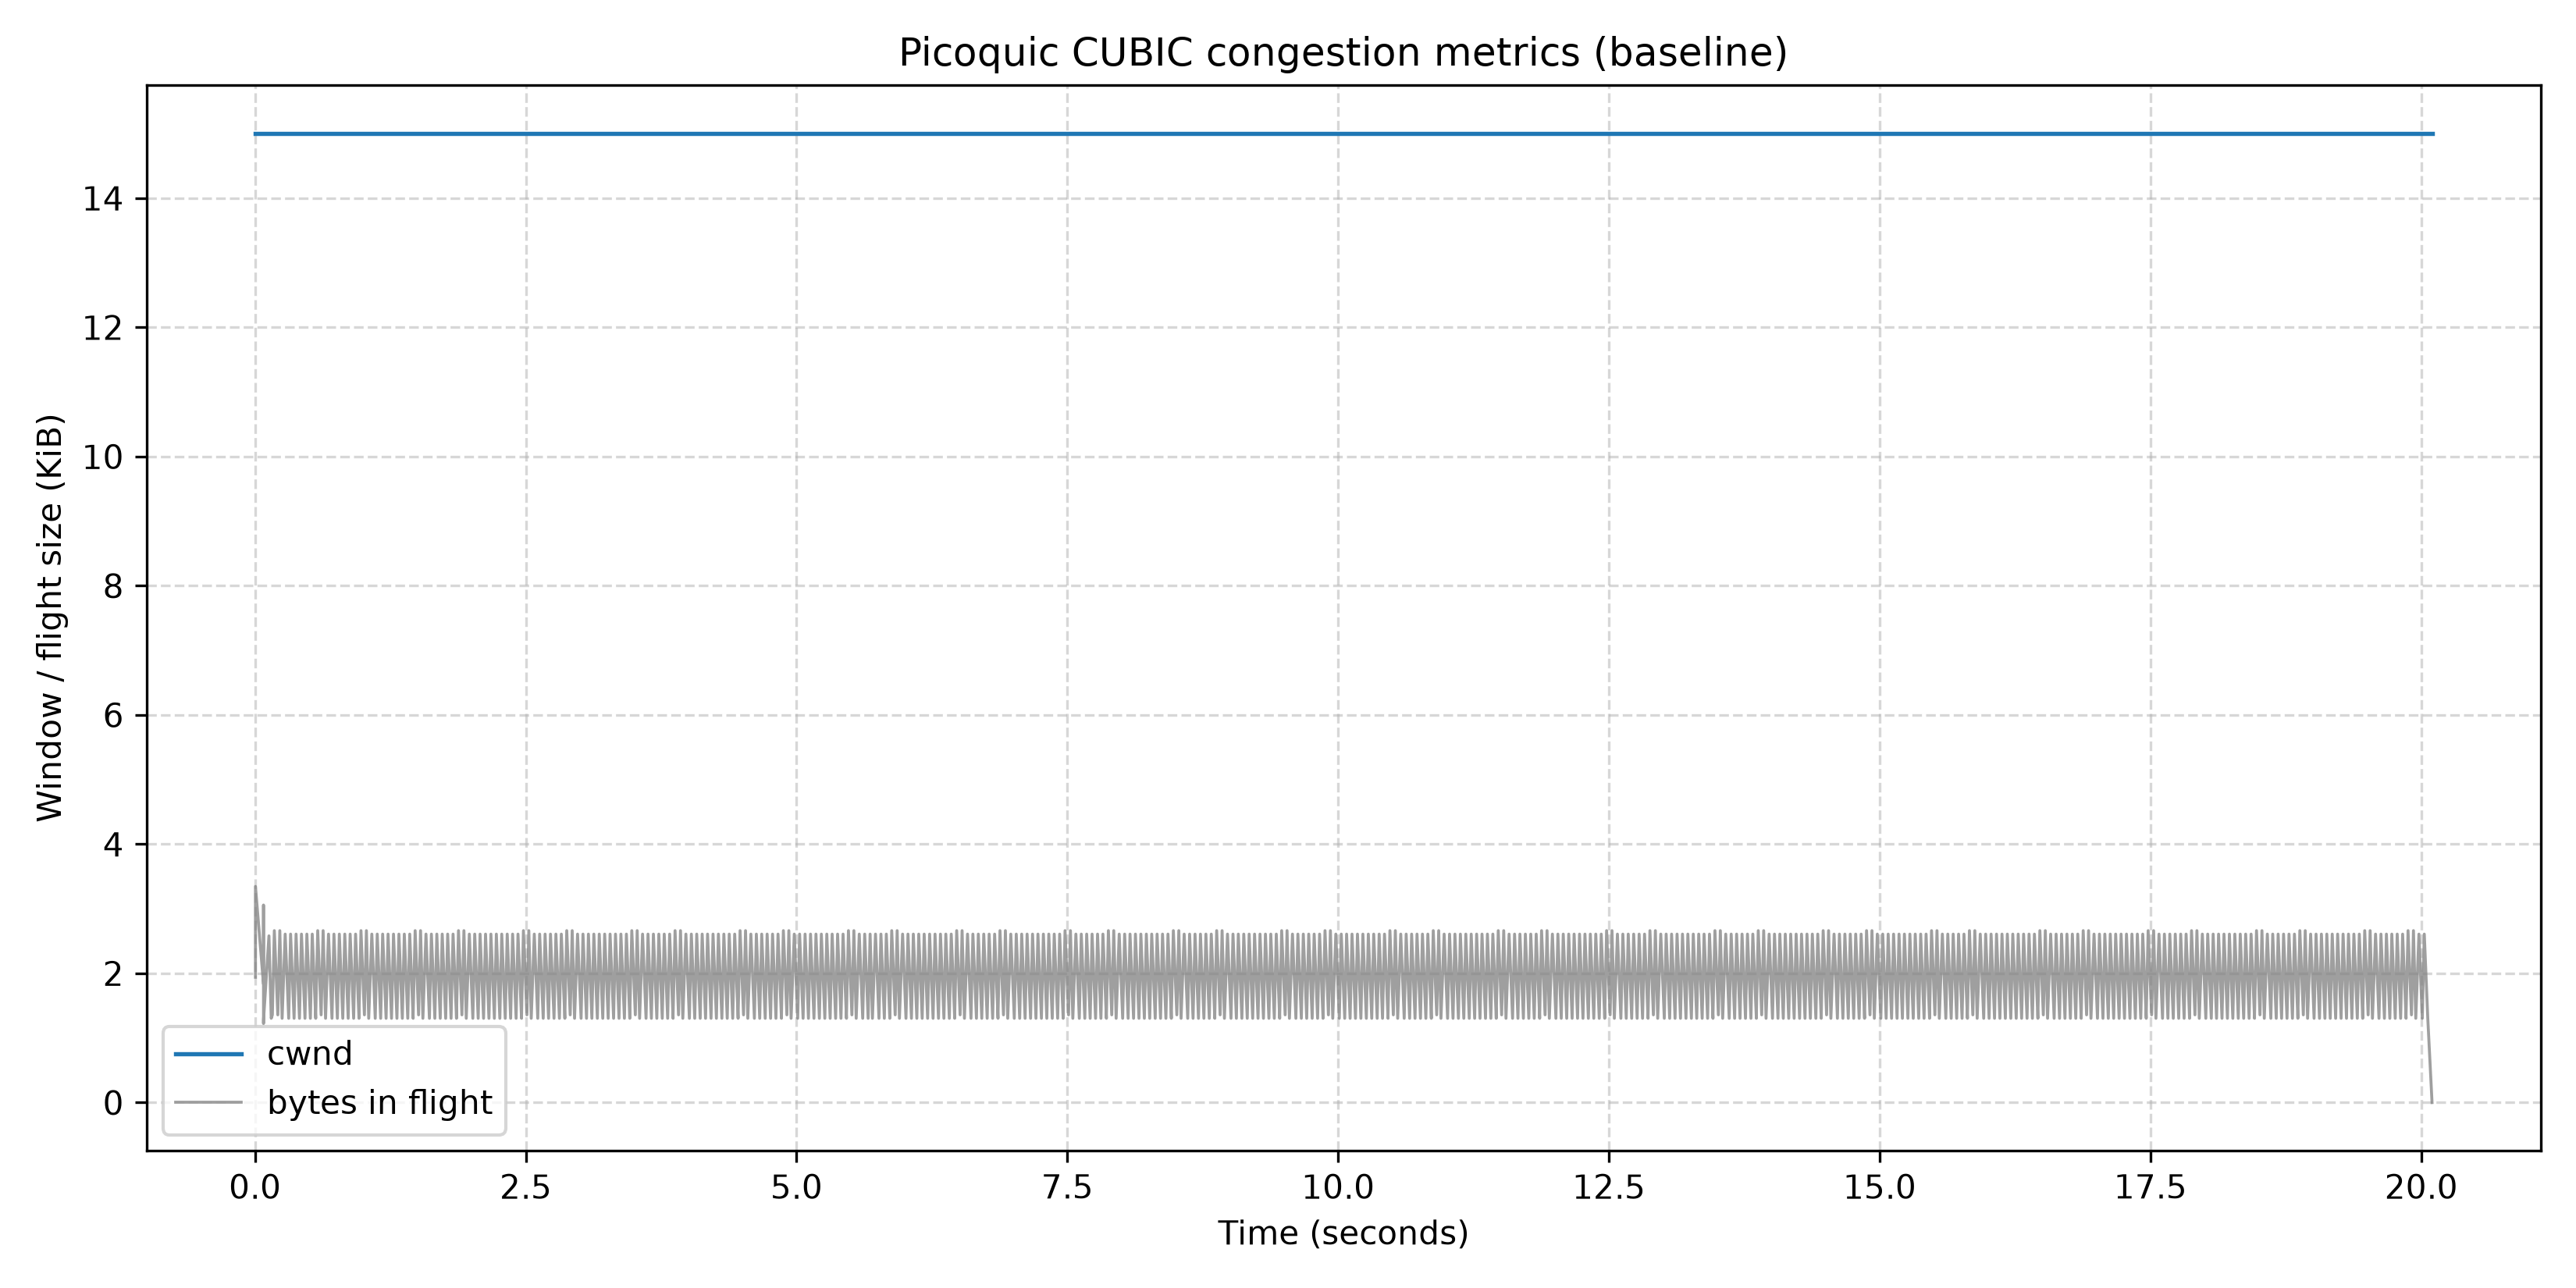
\includegraphics[width=\linewidth,height=.25\textheight,keepaspectratio]{images/native-rate-limited-baseline-1.png}
\captionof{figure}{Original CUBIC, fresh fixed-rate repetition one.}
\end{center}
\begin{center}
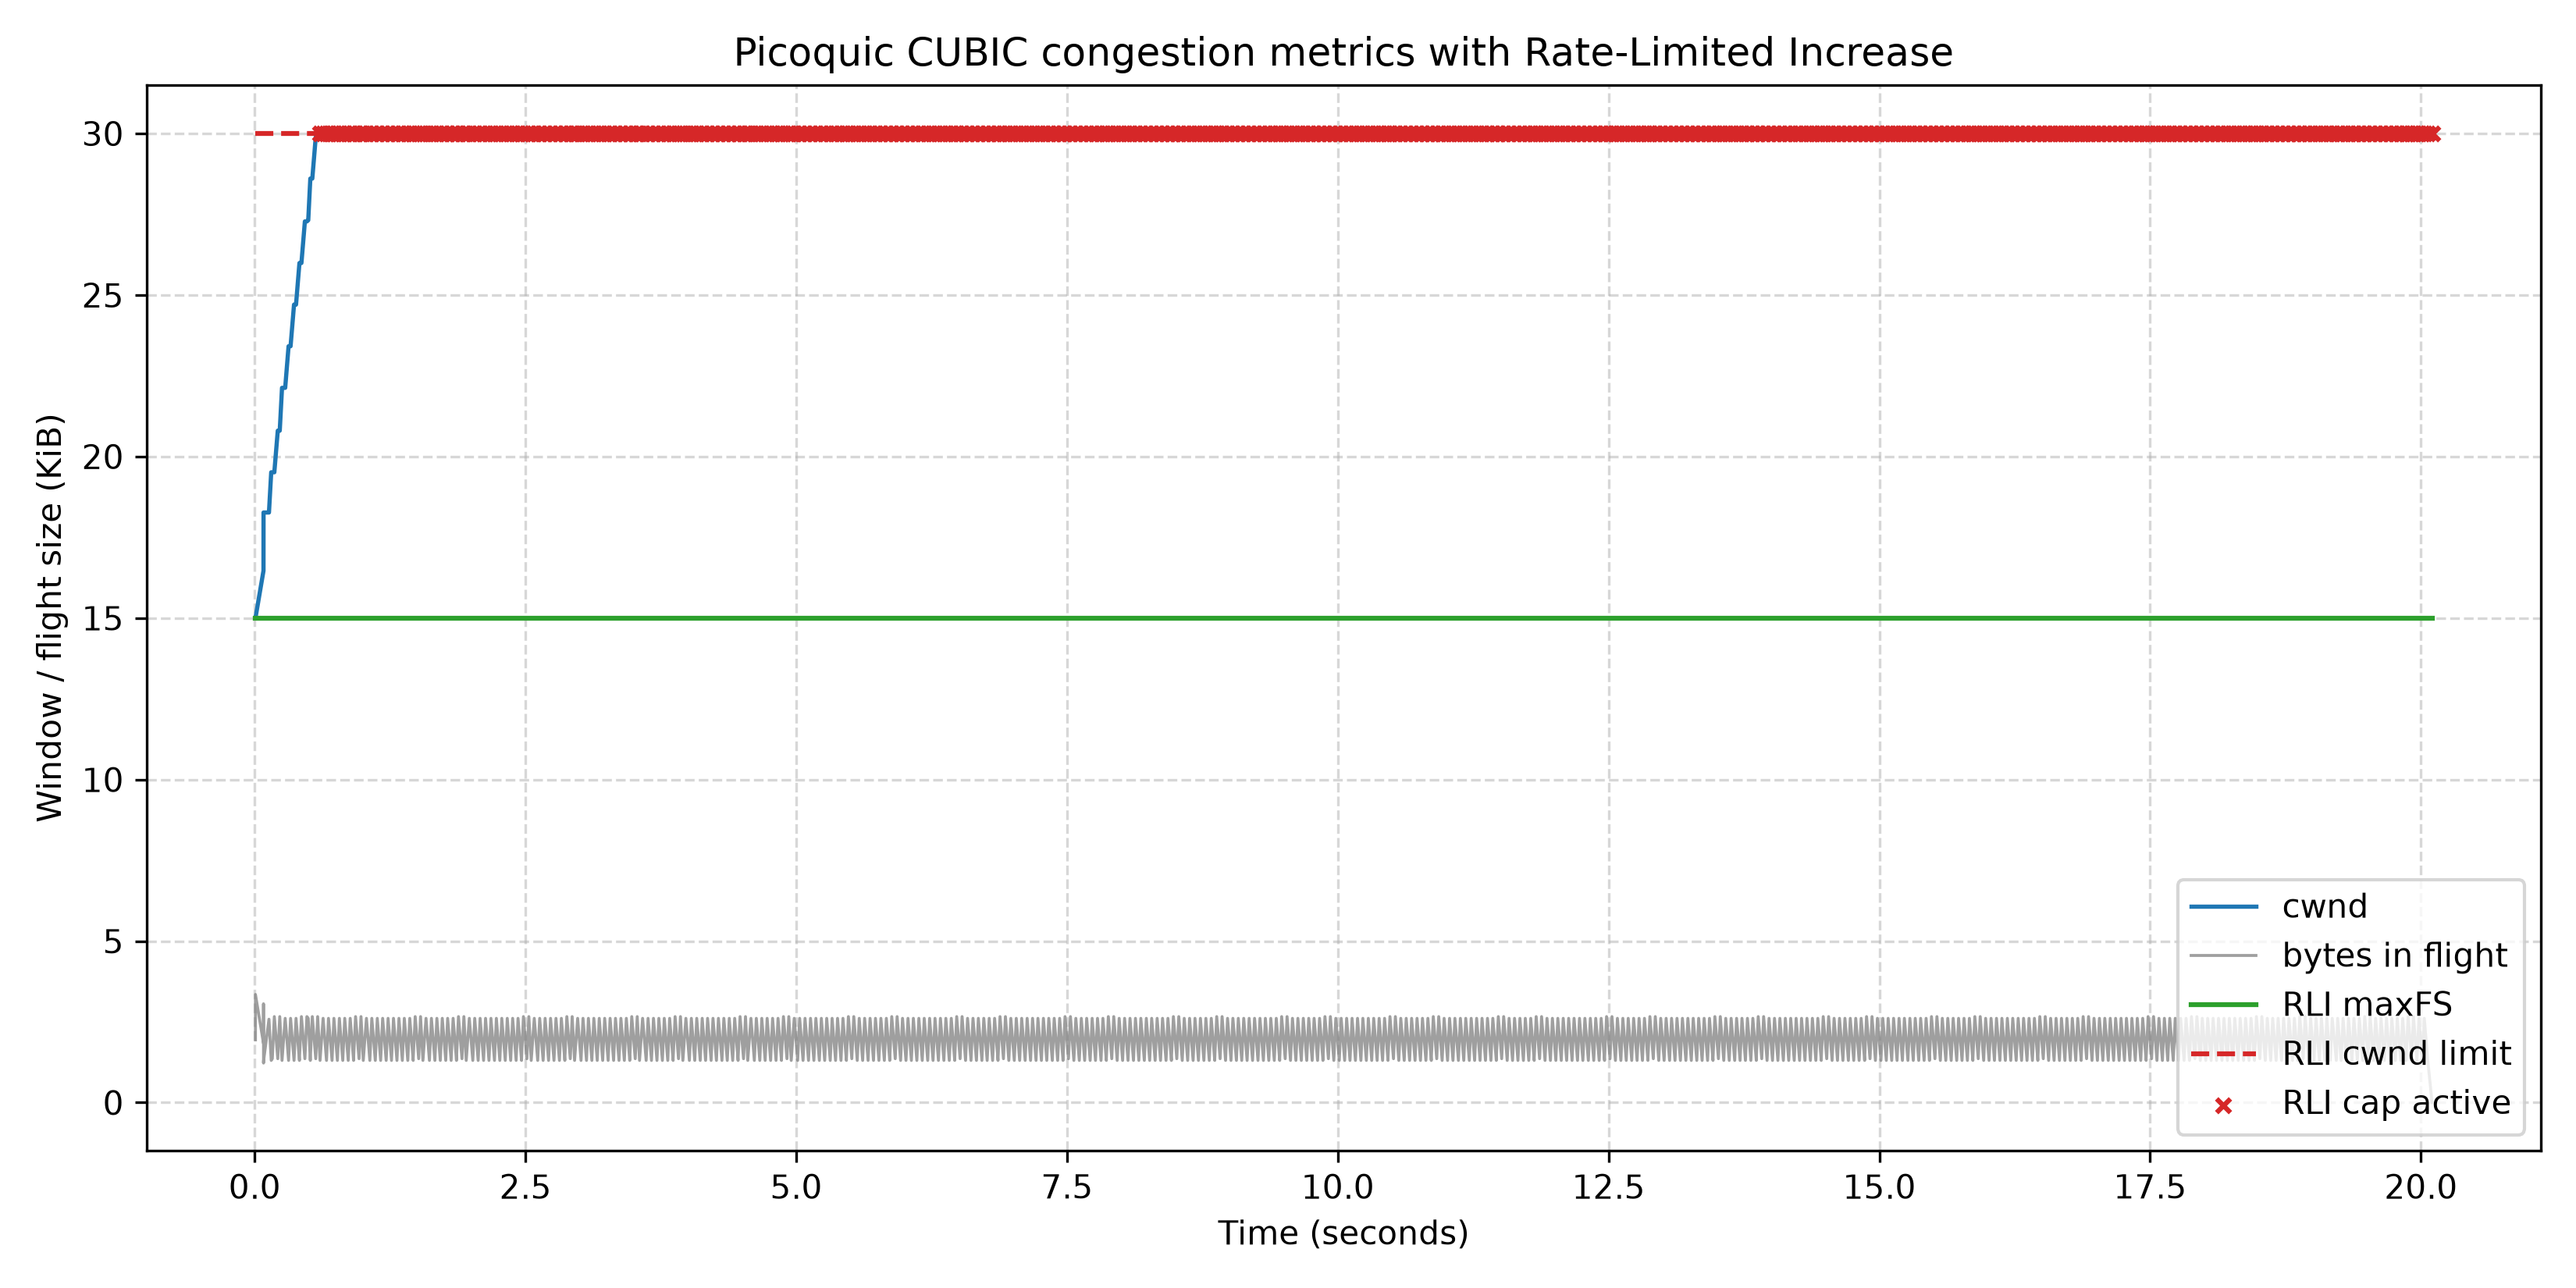
\includegraphics[width=\linewidth,height=.25\textheight,keepaspectratio]{images/native-rate-limited-rli-1.png}
\captionof{figure}{CUBIC with RLI, fresh fixed-rate repetition one.}
\end{center}

\subsection*{5.3 Single-flow bulk transfers}
\begin{center}\small\begin{tabular}{lrrrr}
Mode & Rate (Mbit/s) & Final cwnd (KiB) & Mean cwnd (KiB) & Final RTT (ms) \\ \hline
Original & 17.096857 & 554.94 & 504.39 & 211.599 \\
RLI & 17.602599 & 358.20 & 286.78 & 139.168 \\
\end{tabular}\end{center}

The observed mean throughput change is +2.96\%.
Paired RLI-minus-baseline differences are +0.449, +0.232, +0.836 Mbit/s.
Three repetitions describe this configuration; they do not establish a general performance gain or regression.
Final smoothed RTT is an endpoint statistic, not a direct queue-occupancy measurement.
The twelve single-flow runs record 0 retransmissions in total.
\begin{center}
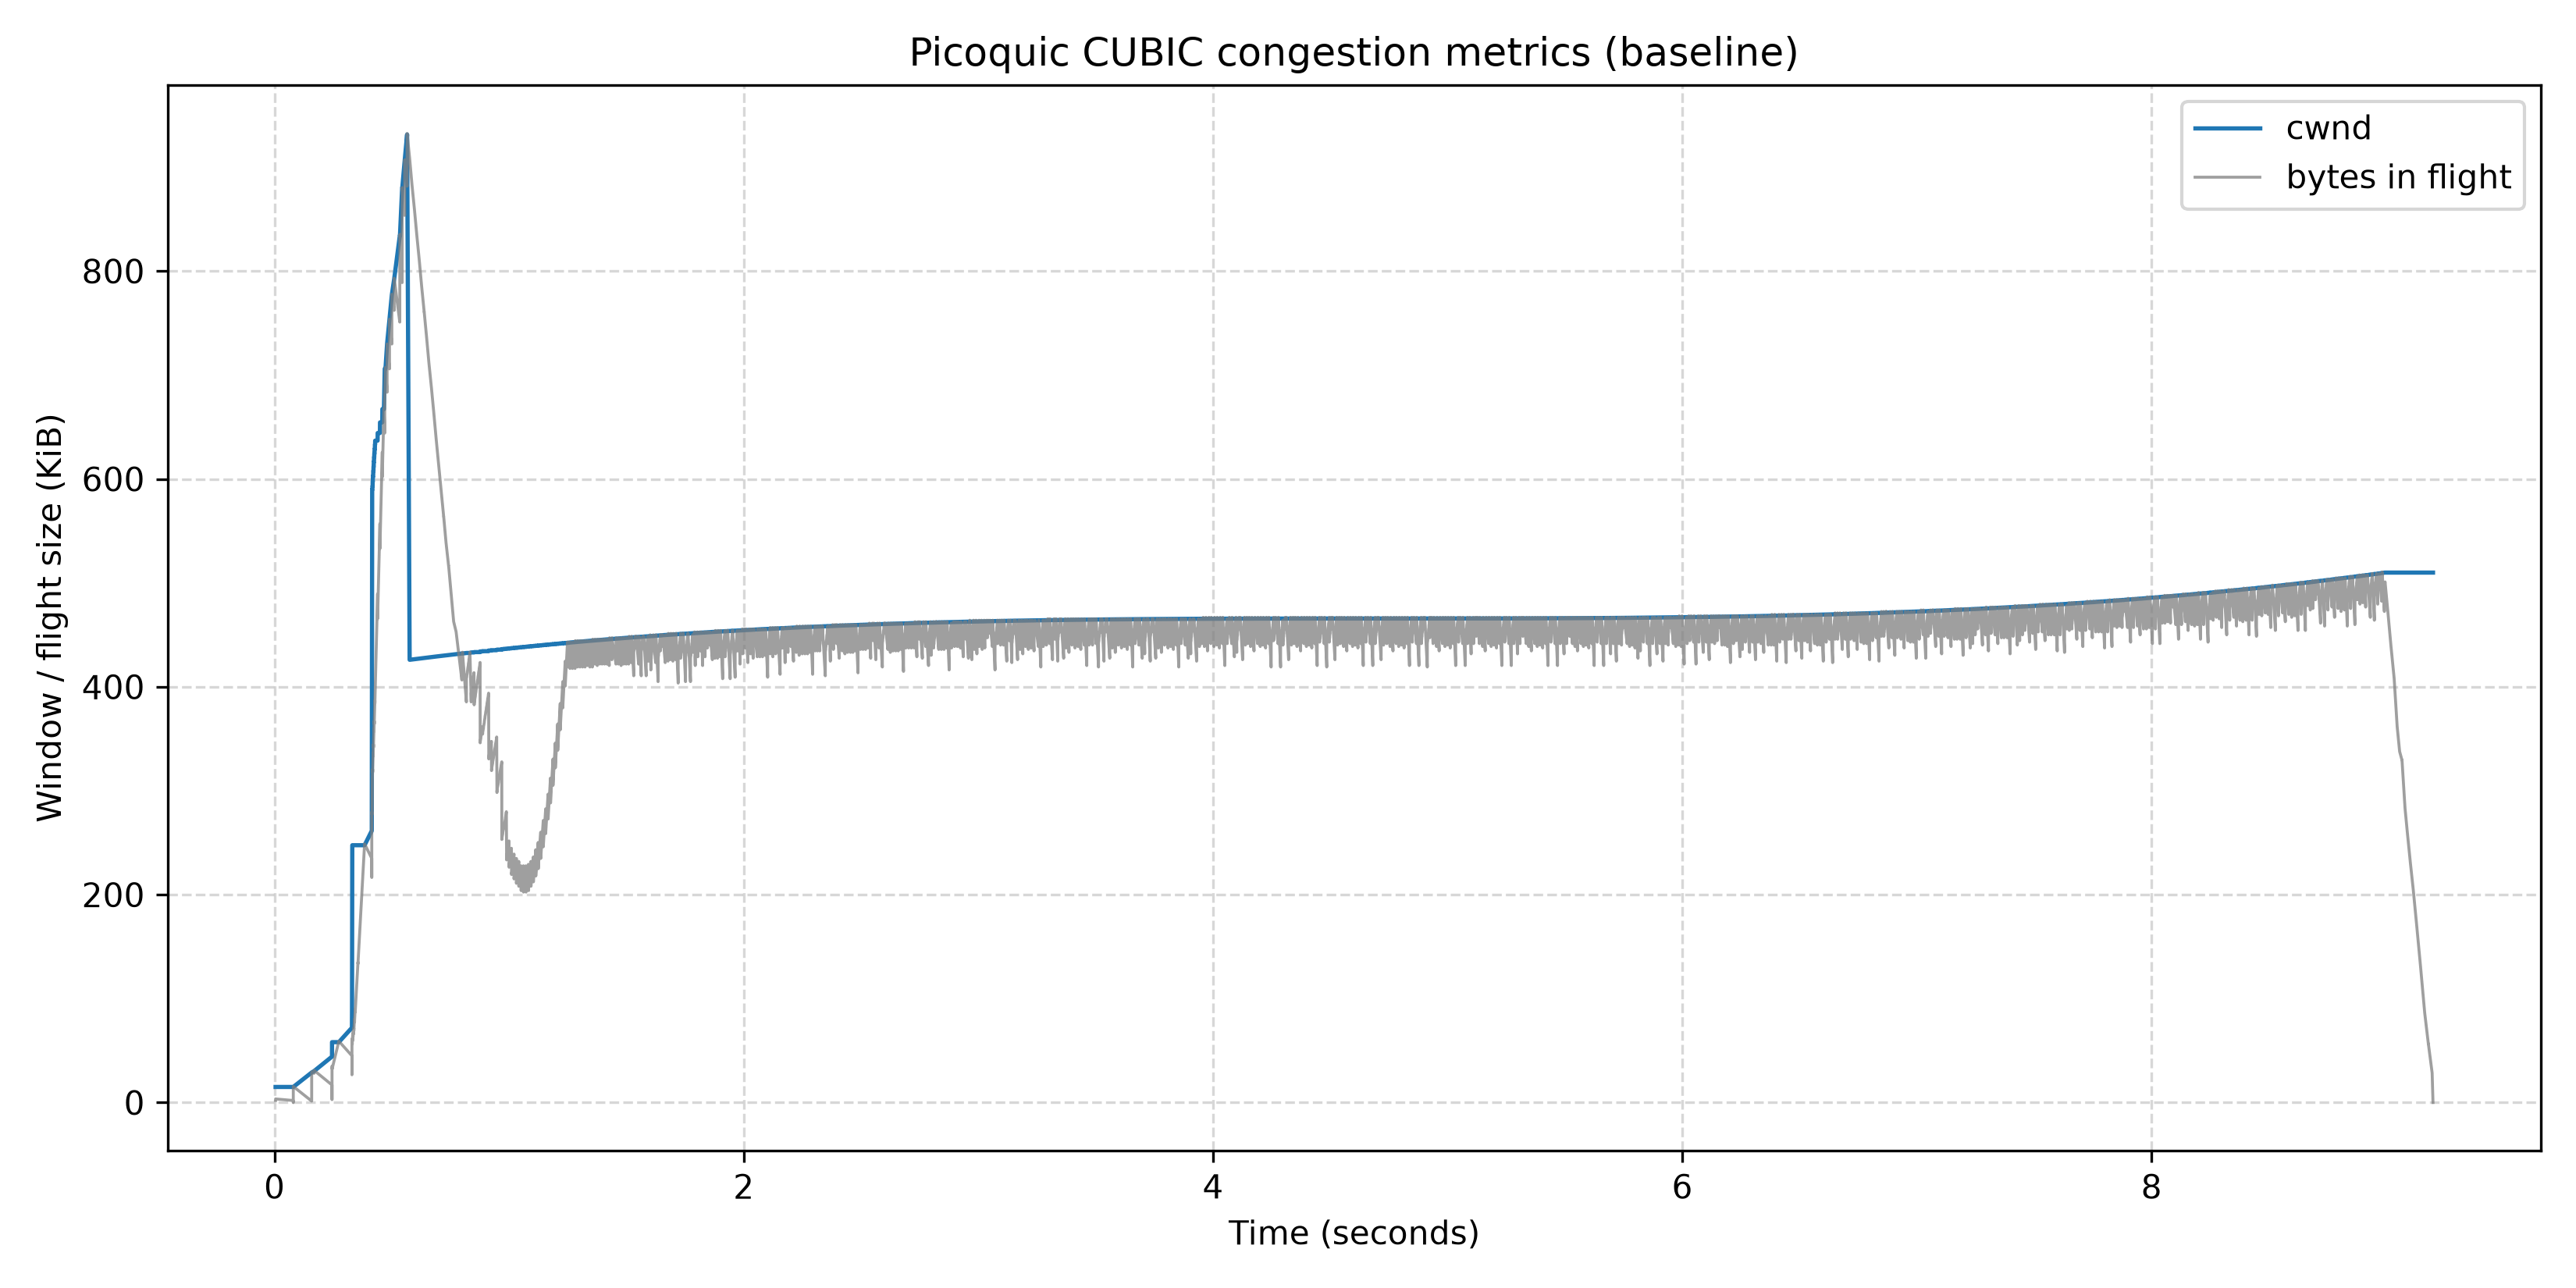
\includegraphics[width=\linewidth,height=.25\textheight,keepaspectratio]{images/native-bulk-baseline-1.png}
\captionof{figure}{Original CUBIC, fresh bulk repetition one.}
\end{center}
\begin{center}
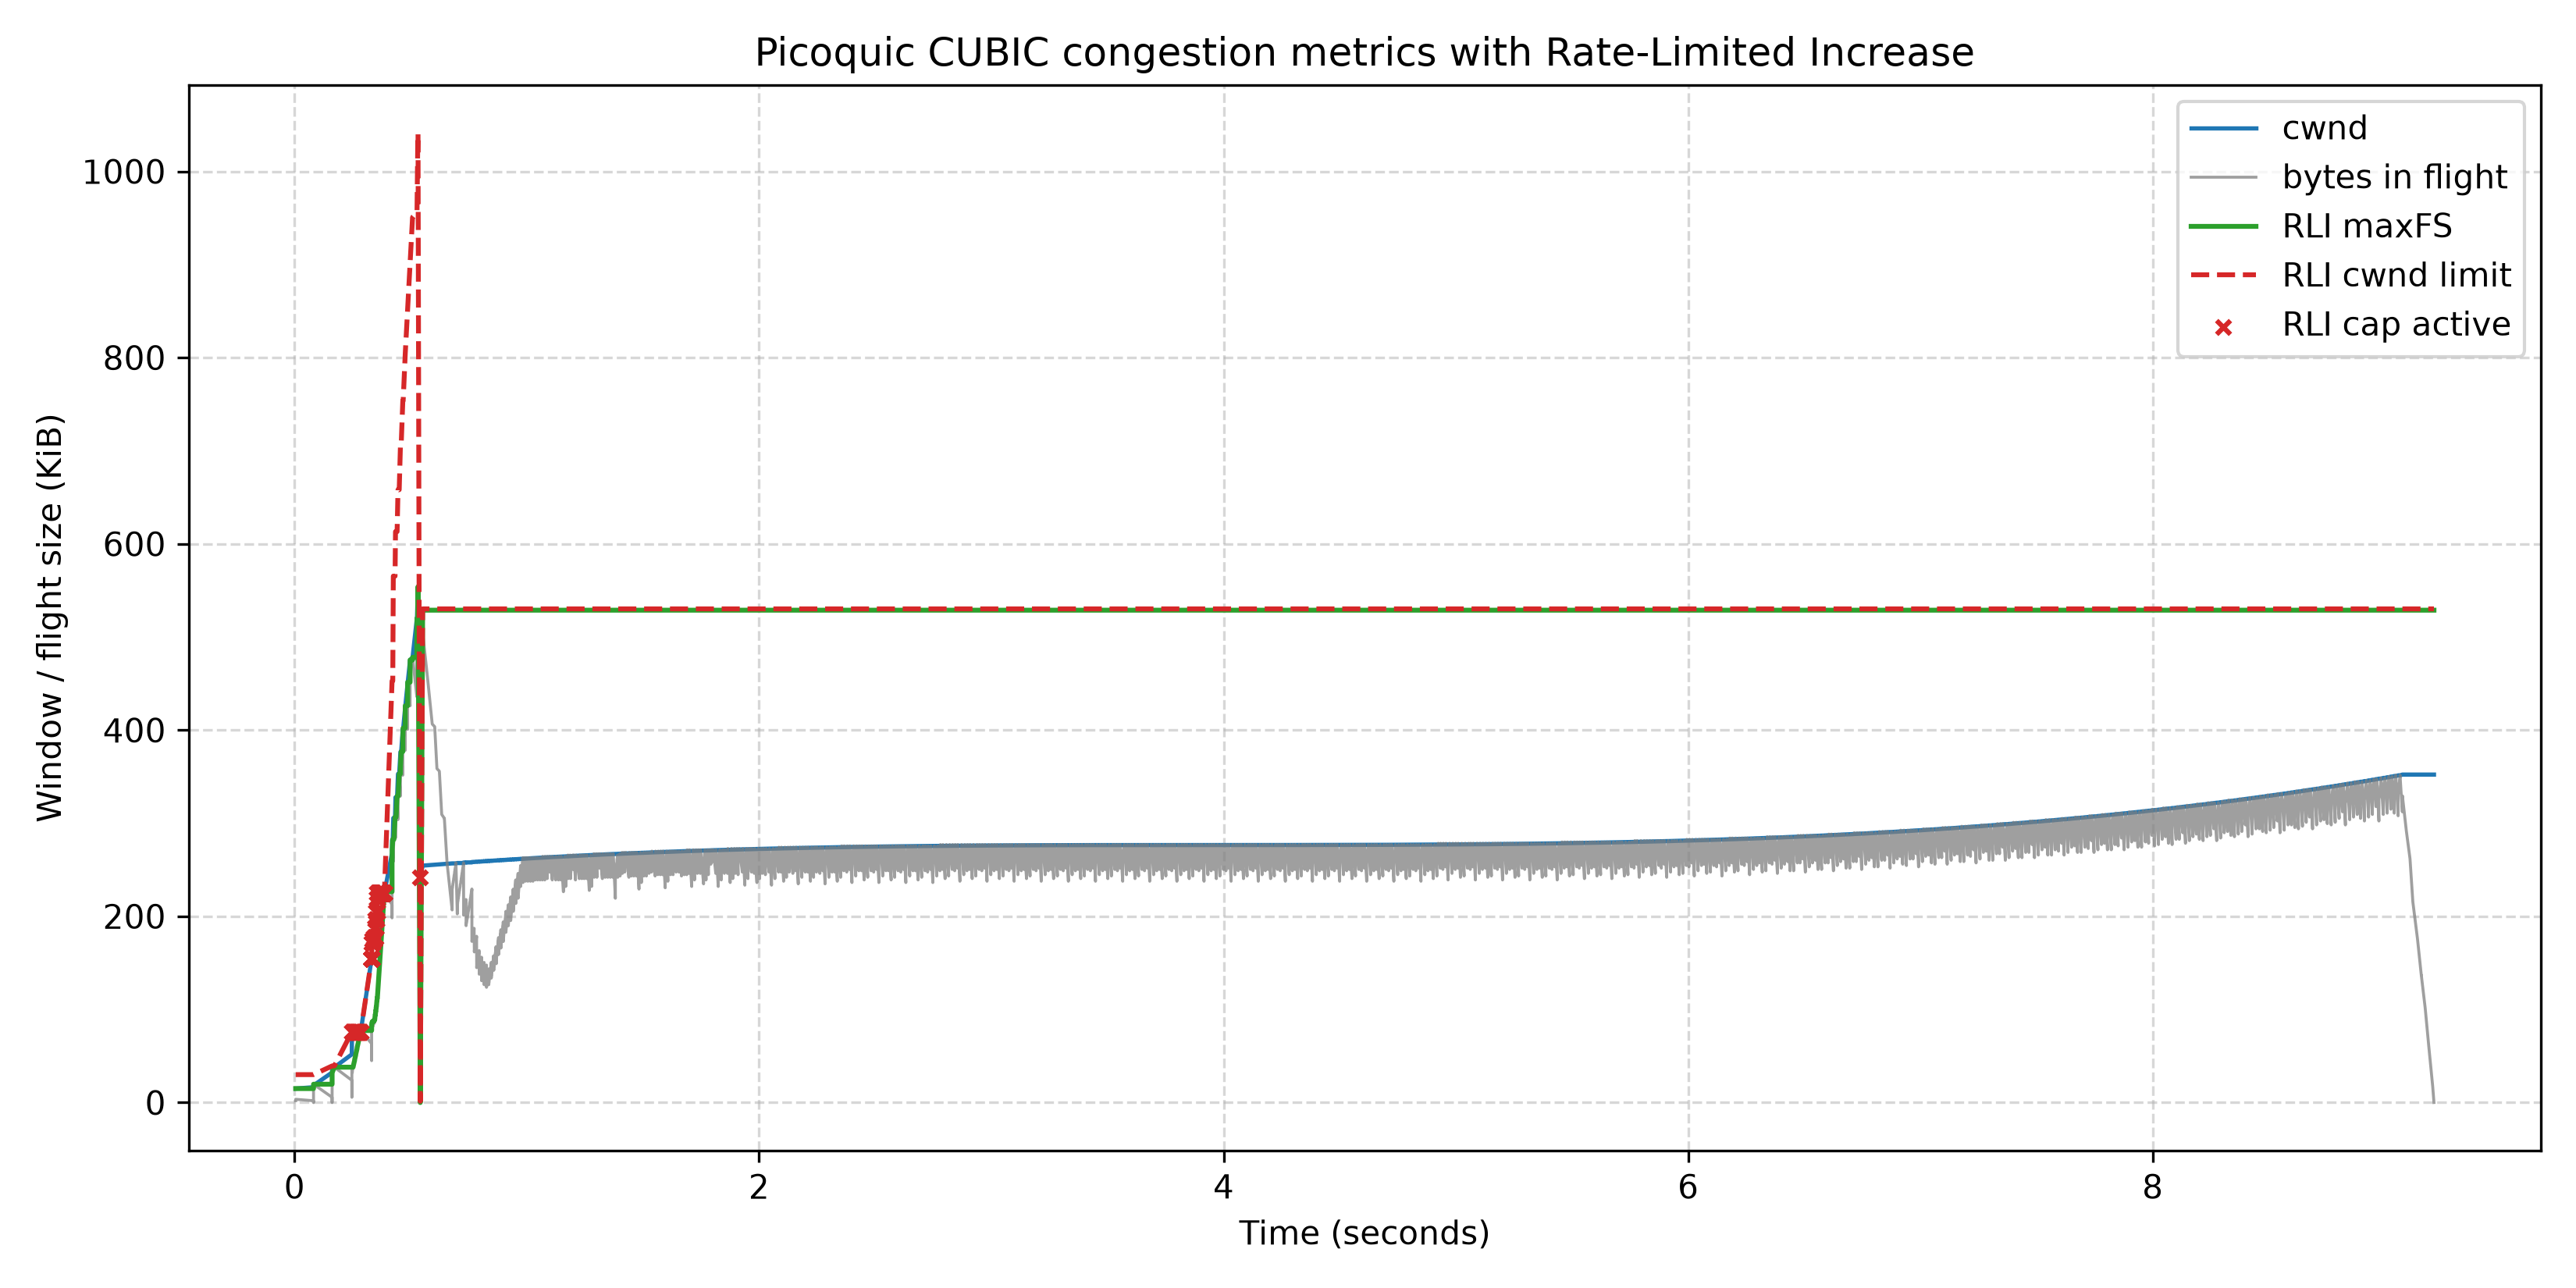
\includegraphics[width=\linewidth,height=.25\textheight,keepaspectratio]{images/native-bulk-rli-1.png}
\captionof{figure}{CUBIC with RLI, fresh bulk repetition one.}
\end{center}

\subsection*{5.4 Two flows sharing the dumbbell}
\begin{center}\small\begin{tabular}{lrrr}
Mode & Combined Mbit/s & Jain index & Mean retransmissions \\ \hline
Original & 18.596 & 0.98700 & 190.3 \\
RLI & 18.580 & 0.98910 & 0.0 \\
\end{tabular}\end{center}

Combined throughput uses the interval from client launch until both clients exit.
Each flow's connection rate uses its server's own connection interval.
The Jain index uses those two per-connection rates; it does not measure instantaneous fairness.
Both connections use the same algorithm in each experiment.
The mean combined-throughput change is -0.08\%.
\begin{center}
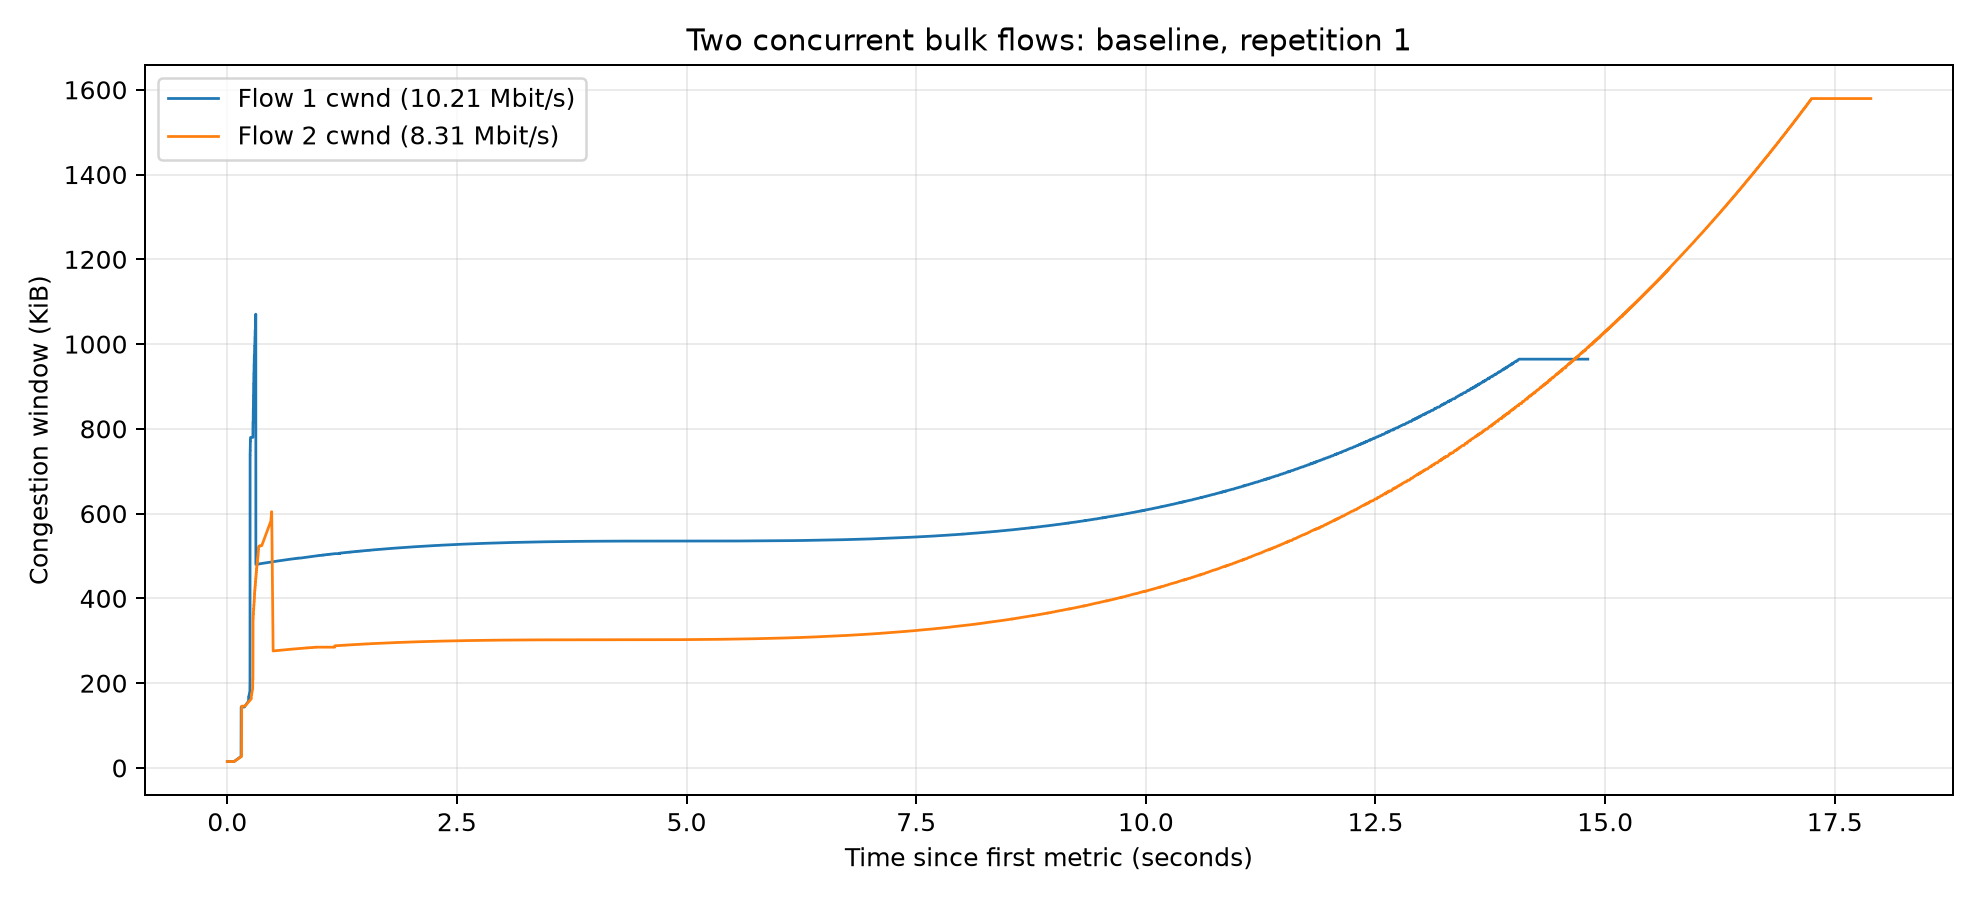
\includegraphics[width=\linewidth,height=.25\textheight,keepaspectratio]{images/native-dumbbell-baseline-1.png}
\captionof{figure}{Two competing flows with original CUBIC, fresh repetition one.}
\end{center}
\begin{center}
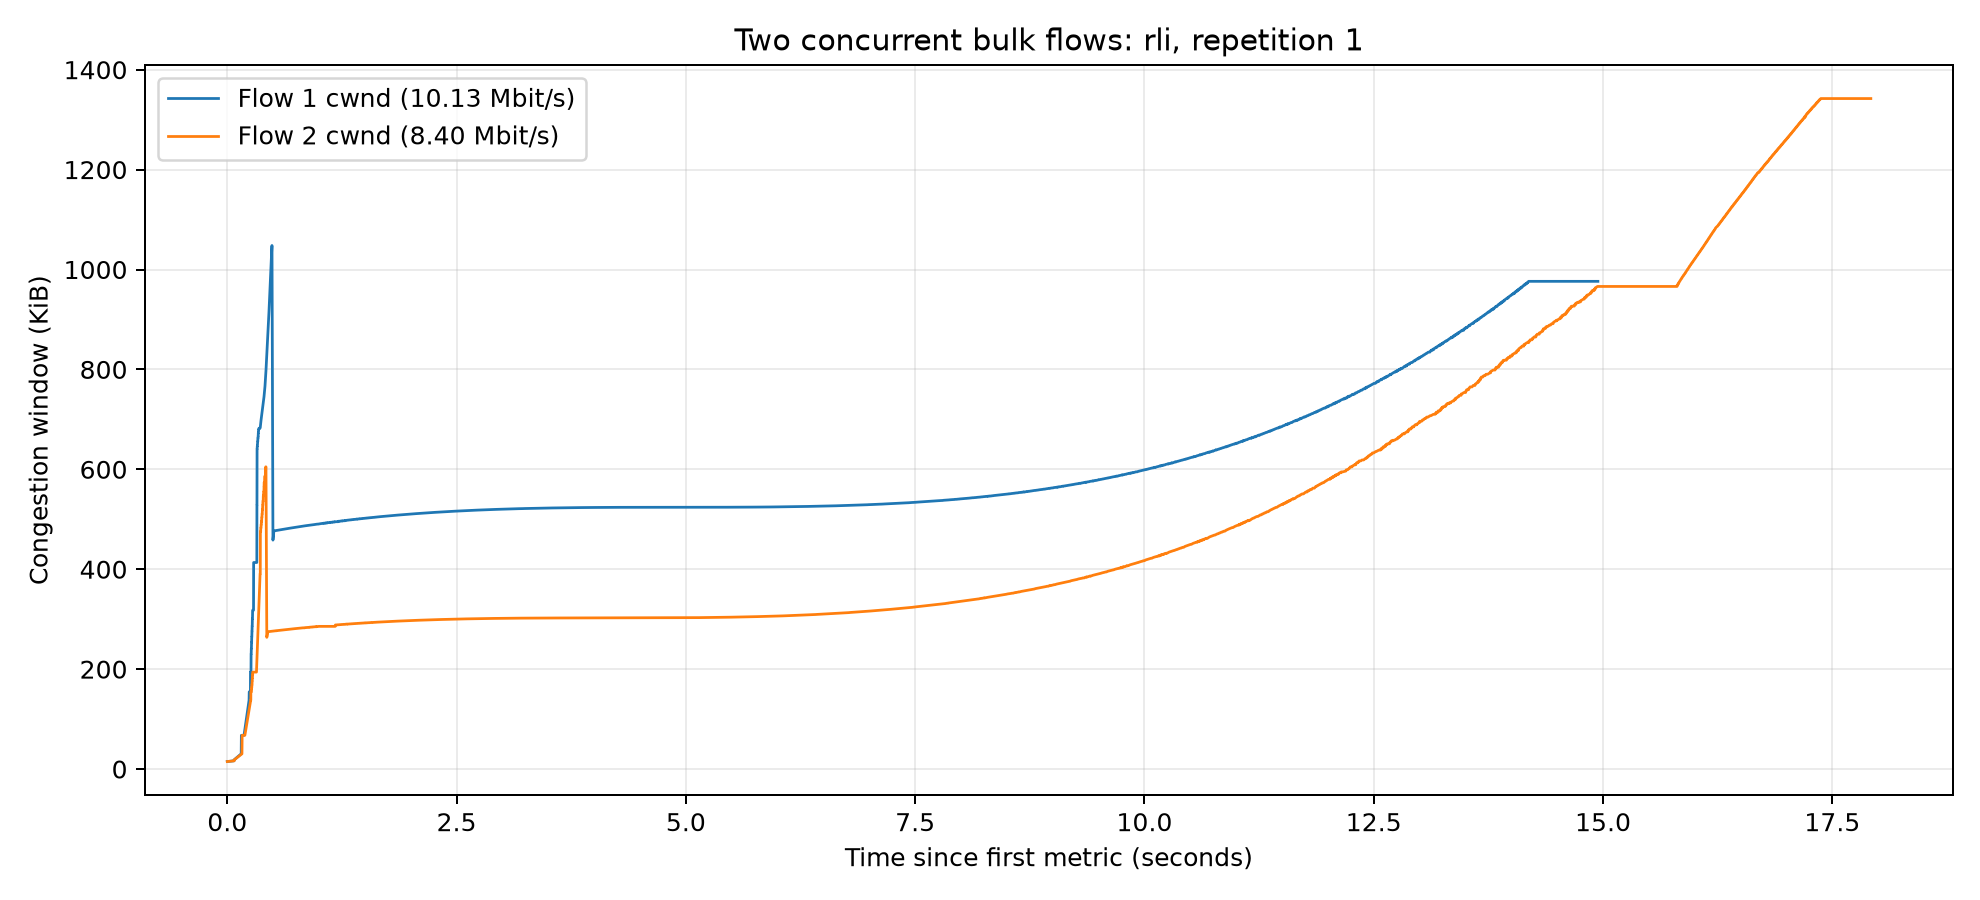
\includegraphics[width=\linewidth,height=.25\textheight,keepaspectratio]{images/native-dumbbell-rli-1.png}
\captionof{figure}{Two competing flows with RLI, fresh repetition one.}
\end{center}

\subsection*{5.5 Validation and comparison}

The current trace validator passes all six single-flow RLI traces and all six competing RLI connections.
Fixed-rate cases require an active cap. RLI bulk cases additionally require a window reduction and an observable flight-history reset.
Both builds pass their registered CTest suites. The separate cubic\_rli test also passes.
Reset counters make history resets observable even when flight size rebuilds between snapshots.

\begin{center}\small
\begin{tabularx}{\linewidth}{@{}p{0.25\linewidth}XX@{}}
\textbf{Aspect} & \textbf{Reference behavior} & \textbf{Observed result}\\ \hline
Application limitation & RFC 9438 suppresses growth in application-limited intervals \cite{ref2}. & RLI grows cwnd from 15 to 30 KiB at the slow-start cap.\\[3pt]
Growth bound & The RLI draft bounds increases using flight history \cite{ref1}. & Fixed-rate runs exercise the slow-start cap. The focused test checks the selected congestion-avoidance cap.\\[3pt]
Window retention & RFC 7661 considers windows that have not been exercised \cite{ref6}. & These experiments evaluate bounded growth, not window aging.\\
\end{tabularx}
\end{center}
\label{sec:results-end}
